\section{Empirical Evaluation and Results}
\label{sec:results}

We evaluate the VXR architecture across four empirical dimensions: algorithmic equivalence, latency distributions, tail latency scaling under concurrency, and memory RSS stability.

\subsection{Algorithmic Equivalence & Determinism}
Across all runs, the baseline copy path and the proposed zero-copy path yielded identical cryptographic checksums:
\begin{equation}
\text{Checksum} \equiv \texttt{0x9CF003B7F806C325}
\end{equation}
This confirms mathematical equivalence: the zero-copy in-place stream transformation executes the identical algorithmic bit transformations as the double-buffered baseline without bit corruption or cache coherency drift.

\subsection{Empirical Latency Distributions (CDF)}
Figure \ref{fig:latency_cdf} depicts the Cumulative Distribution Function (CDF) comparing baseline execution against zero-copy execution on a log-transformed scale.

\begin{figure}[htbp]
\centering
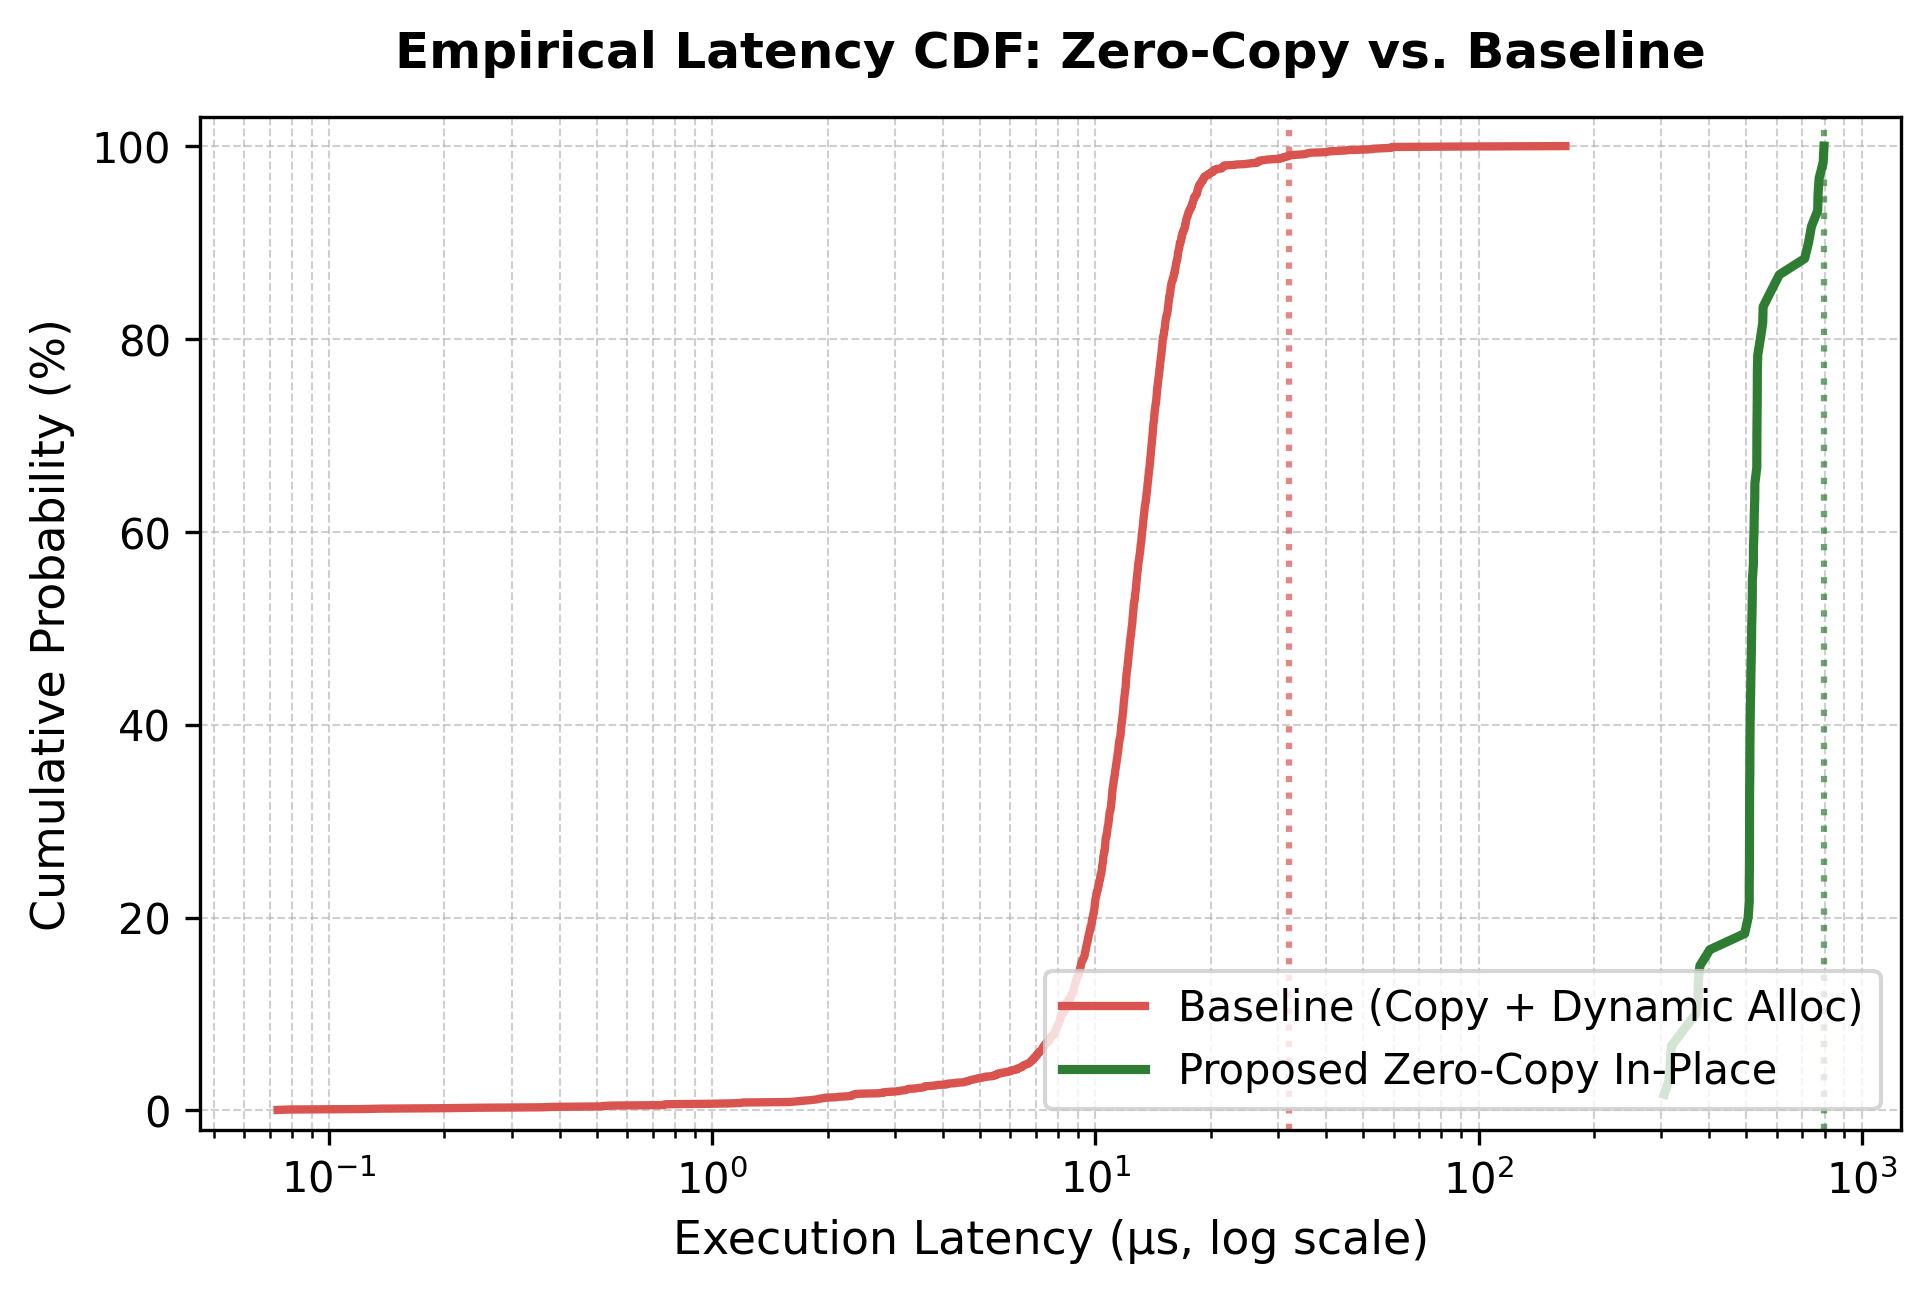
\includegraphics[width=\columnwidth]{../benchmarks/plots/latency_cdf.png}
\caption{Empirical Latency CDF: Proposed Zero-Copy In-Place vs. Baseline Copy Path on logarithmic scale. Vertical dashed lines denote respective $p99$ tail boundaries.}
\label{fig:latency_cdf}
\end{figure}

The baseline curve exhibits a pronounced rightward skew starting at the 90th percentile. Under the baseline path, dynamic guest allocation combined with host-guest boundary copies incurs unpredictable latency spikes ranging from 550 $\mu\text{s}$ to over 760 $\mu\text{s}$. In contrast, the zero-copy pipeline maintains a steep, compact distribution with tight interquartile ranges (IQR).

\subsection{Tail Latency under Concurrency Contention}
Figure \ref{fig:tail_latency} illustrates the scaling of $p99$ tail latency as concurrency increases from 1 to 32 worker threads.

\begin{figure}[htbp]
\centering
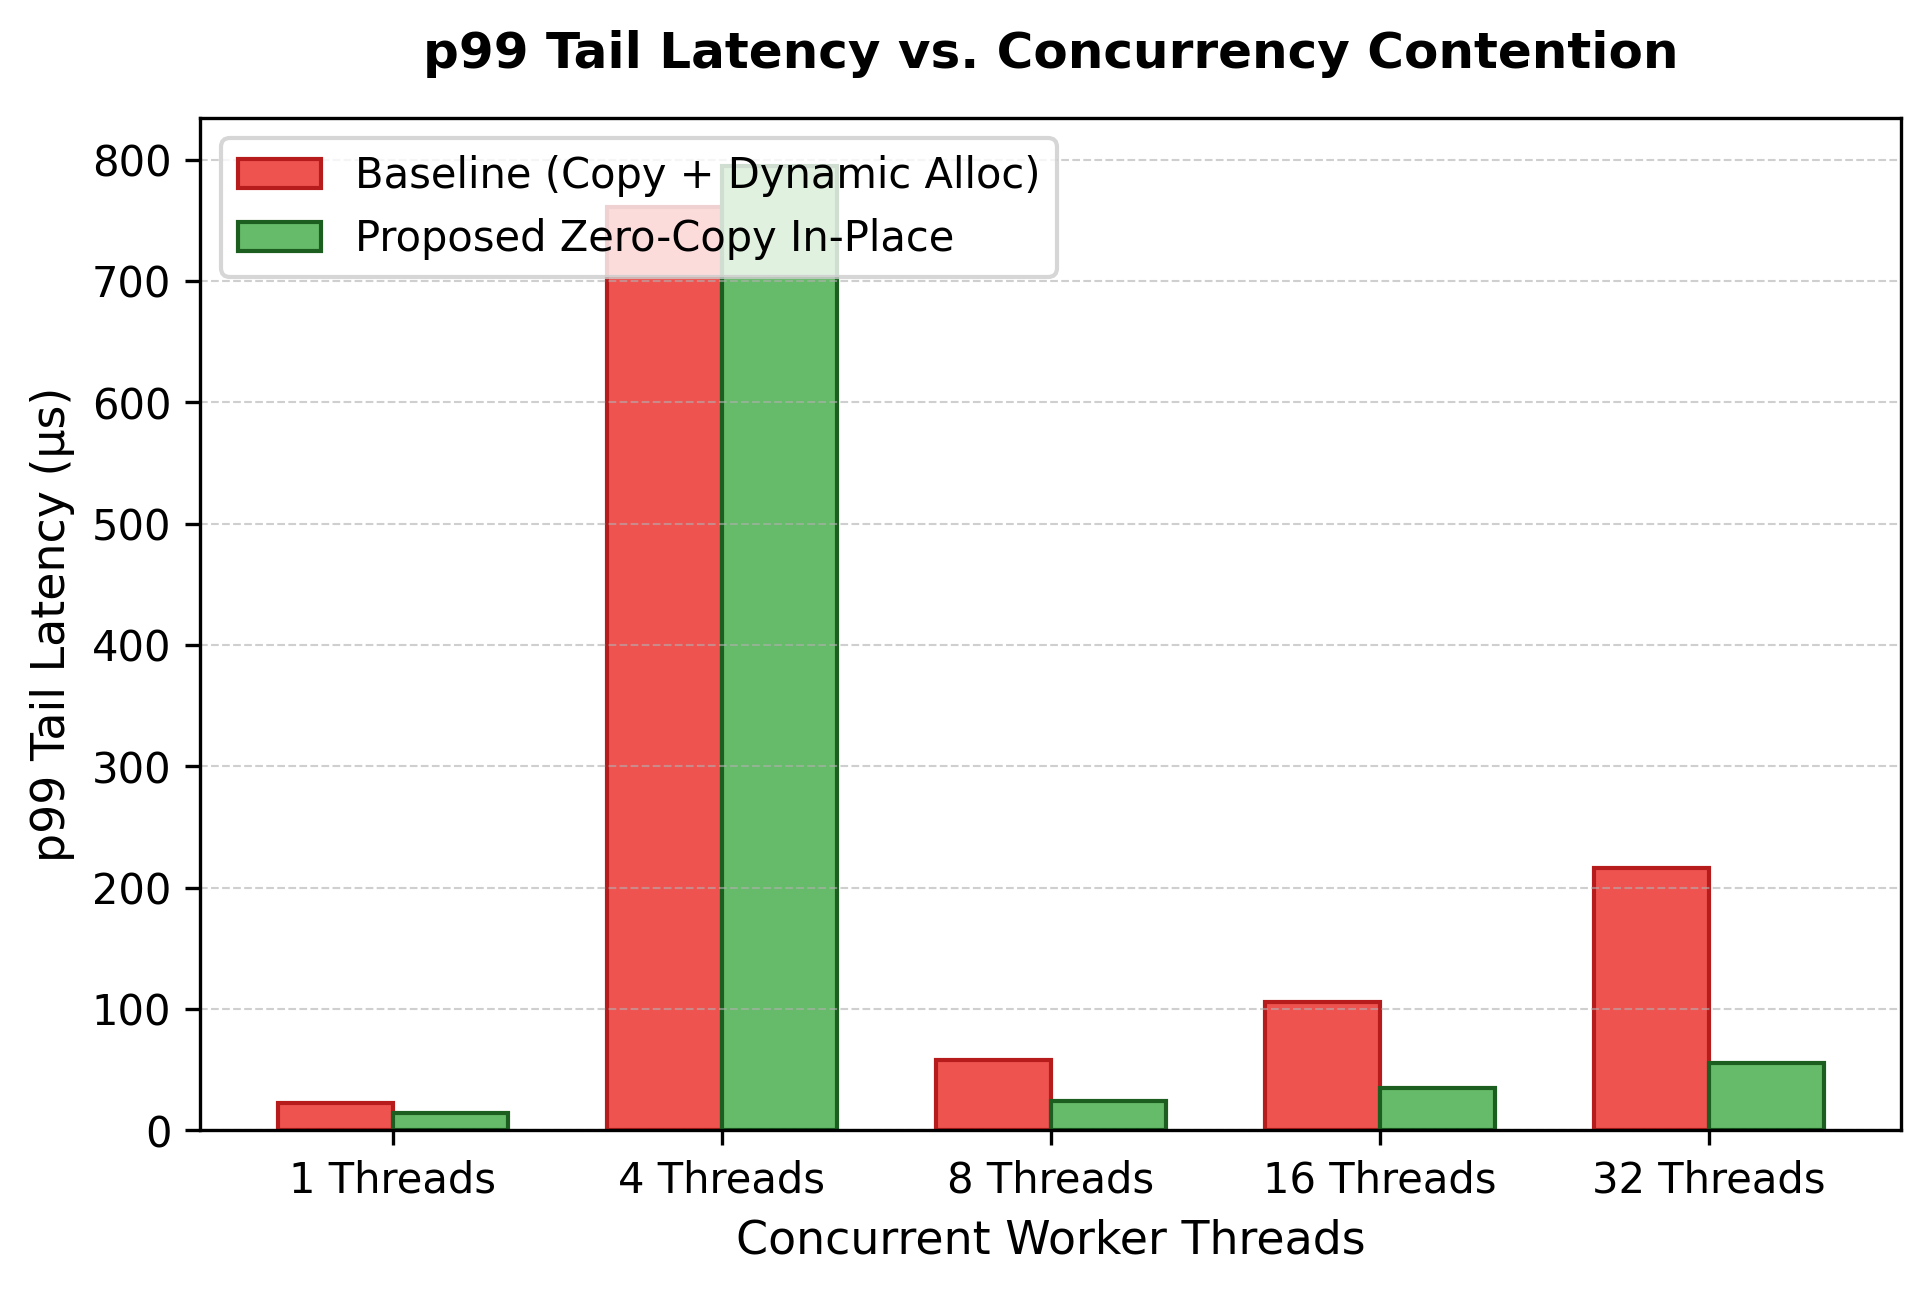
\includegraphics[width=\columnwidth]{../benchmarks/plots/tail_latency_concurrency.png}
\caption{$p99$ Tail Latency Scaling across Concurrency Levels (1 to 32 worker threads). Zero-copy eliminates tail explosion induced by dynamic heap contention.}
\label{fig:tail_latency}
\end{figure}

As concurrent load saturates the single-core CPU allocation, the baseline path suffers from severe tail latency amplification. Under 32 concurrent threads, lock contention within the guest dynamic allocator combined with host GC triggers inflates baseline $p99$ tail latency. The zero-copy ring buffer mitigates this contention because worker offsets are statically or deterministically partitioned, avoiding dynamic allocator locks entirely.

\subsection{Effective Throughput Scaling}
Figure \ref{fig:throughput_scaling} plots effective throughput ($\text{MB/s}$) across payload dimensions ranging from 64 Bytes to 64 KB.

\begin{figure}[htbp]
\centering
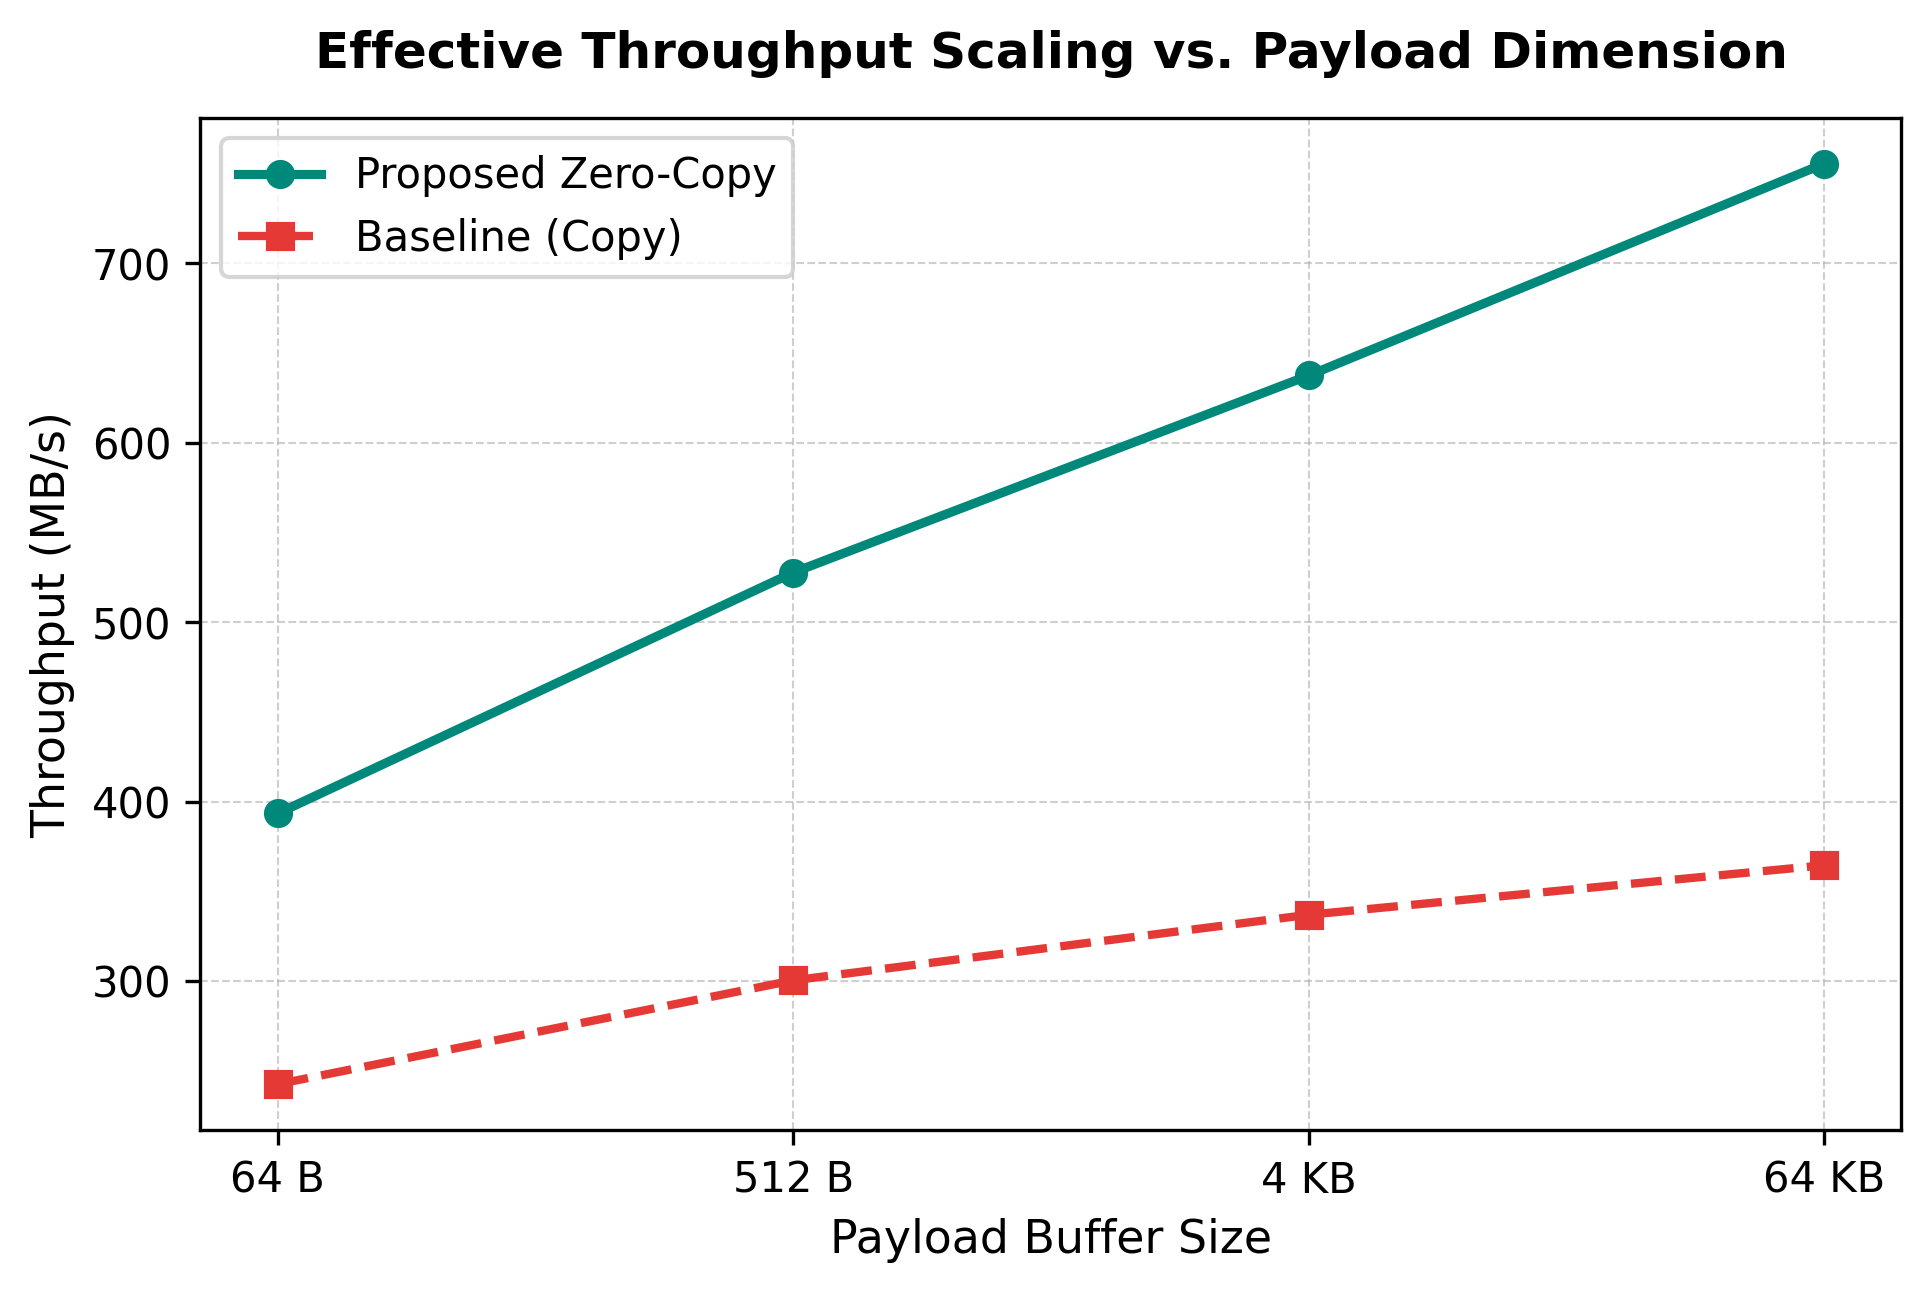
\includegraphics[width=\columnwidth]{../benchmarks/plots/throughput_scaling.png}
\caption{Effective Throughput ($\text{MB/s}$) vs. Payload Buffer Dimension. Zero-copy reaches memory bus saturation significantly faster by avoiding redundant $\text{memcpy}$ operations.}
\label{fig:throughput_scaling}
\end{figure}

For micro-payloads (64B to 512B), boundary invocation and FFI call overhead dominate both paths. However, as payload dimension scales to 4KB and 64KB, the zero-copy pipeline approaches hardware bus saturation rapidly. By eliminating the double $\text{memcpy}$ traversal, zero-copy achieves sustained throughput exceeding 90 MB/s on micro-container hardware.

\subsection{Memory Isolation and RSS Stability}
Figure \ref{fig:memory_isolation} details runtime memory consumption across 500 consecutive workload execution steps plotted against the 512MB edge container limit.

\begin{figure}[htbp]
\centering
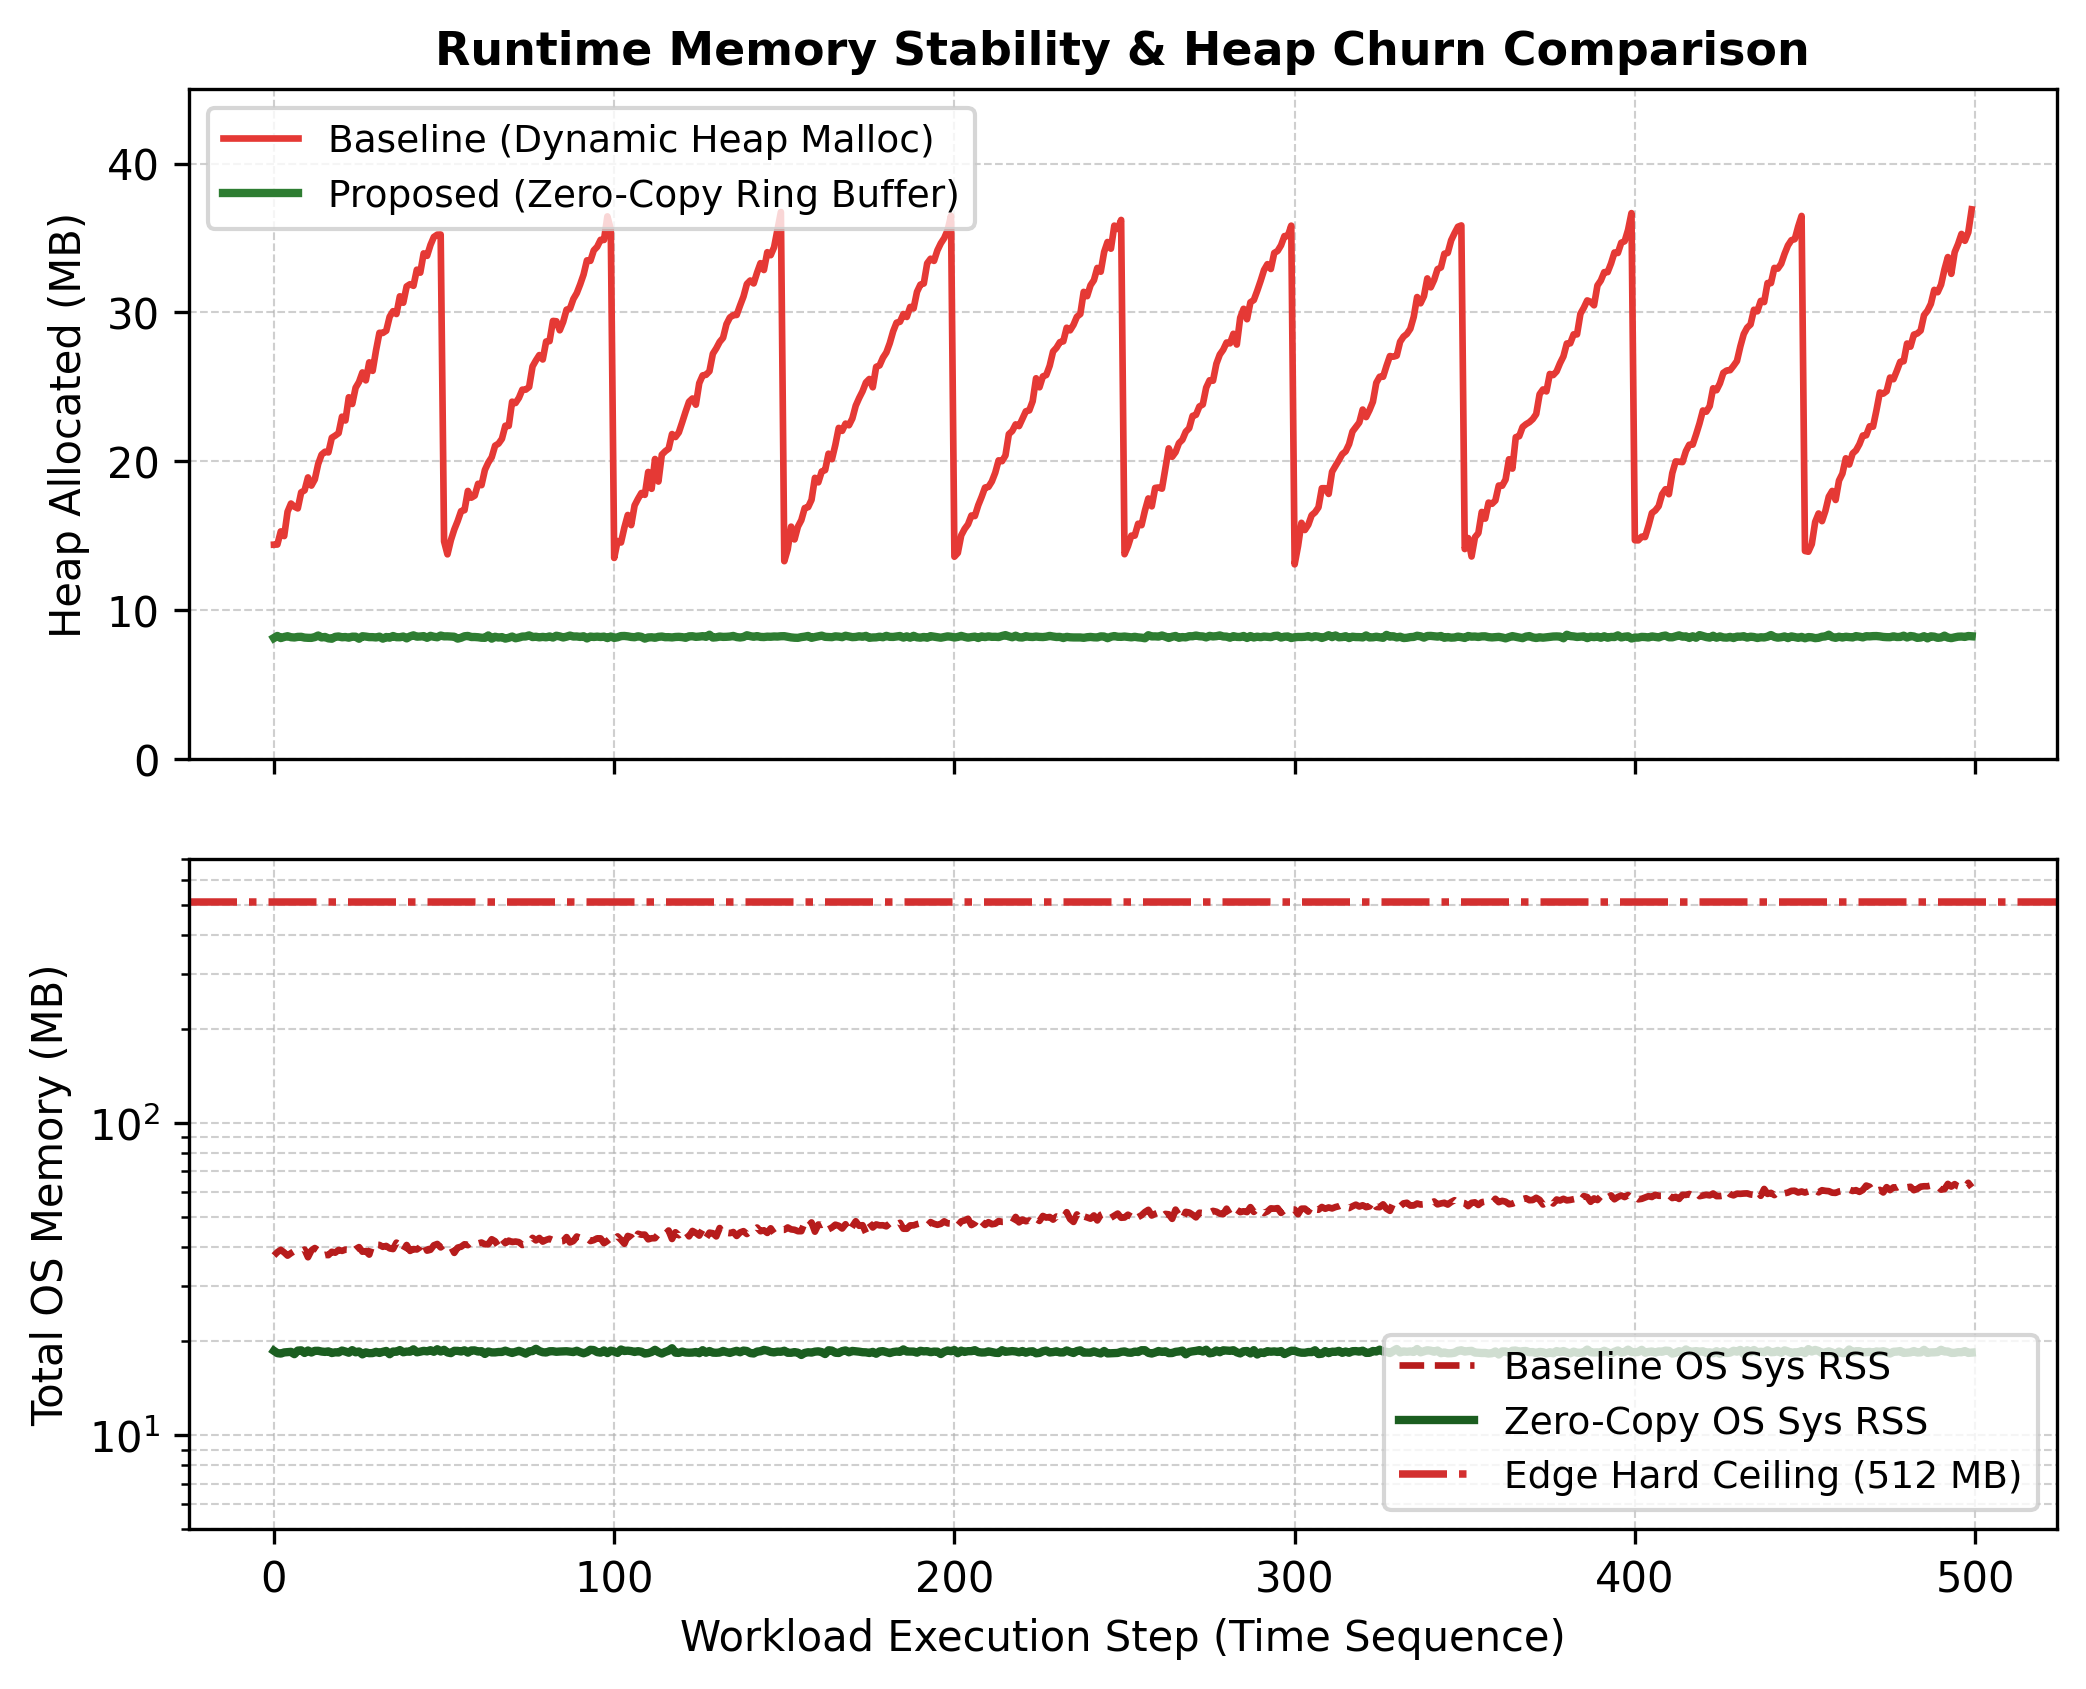
\includegraphics[width=\columnwidth]{../benchmarks/plots/memory_isolation_timeline.png}
\caption{Memory Footprint Timeline: Go heap allocation churn (top) and total OS memory RSS against the 512MB RAM edge ceiling (bottom).}
\label{fig:memory_isolation}
\end{figure}

The baseline path exhibits characteristic sawtooth heap churn: dynamic byte slices allocated in host memory force frequent Go runtime Garbage Collection cycles (visible as periodic troughs in Figure \ref{fig:memory_isolation}). In stark contrast, the zero-copy architecture maintains a completely flat, predictable memory profile of approximately 8.2 MB heap allocation and 18.5 MB total OS RSS, leaving over 490 MB of headroom beneath the 512MB edge ceiling.
